%%% Template originaly created by Karol Kozioł (mail@karol-koziol.net) and modified for ShareLaTeX use

\documentclass[a4paper,11pt]{article}

\usepackage[T1]{fontenc}
\usepackage[utf8]{inputenc}
\usepackage{graphicx}
\usepackage{xcolor}
\usepackage[]{authblk}
\usepackage{amsmath}

\renewcommand\familydefault{\sfdefault}
\usepackage{tgheros}
\usepackage[defaultmono]{droidmono}

\usepackage{amsmath,amssymb,amsthm,textcomp}
\usepackage{enumerate}
\usepackage{multicol}
\usepackage{tikz}

\usepackage{geometry}
%\geometry{total={210mm,297mm},
%left=25mm,right=25mm,%
%bindingoffset=0mm, top=20mm,bottom=20mm}


\linespread{1.2}

\newcommand{\linia}{\rule{\linewidth}{0.5pt}}

% custom theorems if needed
\newtheoremstyle{mytheor}
    {1ex}{1ex}{\normalfont}{0pt}{\scshape}{.}{1ex}
    {{\thmname{#1 }}{\thmnumber{#2}}{\thmnote{ (#3)}}}

%\theoremstyle{mytheor}
%\newtheorem{defi}{Definition}

% my own titles
\makeatletter
\renewcommand{\maketitle}{
\begin{center}
\vspace{2ex}
{\LARGE \textsc{\@title}}
\vspace{1ex}
\\
\linia\\
\@author \hfill October 23, 2017
\vspace{4ex}
\end{center}
}
\makeatother
%%%

% custom footers and headers
\usepackage{fancyhdr}
\pagestyle{fancy}
\lhead{}
\chead{}
\rhead{}
\lfoot{Assignment \textnumero{} 2}
\cfoot{}
\rfoot{Page \thepage}
\renewcommand{\headrulewidth}{0pt}
\renewcommand{\footrulewidth}{0pt}
%

% code listing settings
\usepackage{listings}
\lstset{
    language=Python,
    basicstyle=\ttfamily\small,
    aboveskip={1.0\baselineskip},
    belowskip={1.0\baselineskip},
    columns=fixed,
    extendedchars=true,
    breaklines=true,
    tabsize=4,
    prebreak=\raisebox{0ex}[0ex][0ex]{\ensuremath{\hookleftarrow}},
    frame=lines,
    showtabs=false,
    showspaces=false,
    showstringspaces=false,
    keywordstyle=\color[rgb]{0.627,0.126,0.941},
    commentstyle=\color[rgb]{0.133,0.545,0.133},
    stringstyle=\color[rgb]{01,0,0},
    numbers=left,
    numberstyle=\small,
    stepnumber=1,
    numbersep=10pt,
    captionpos=t,
    escapeinside={\%*}{*)}
}

%%%----------%%%----------%%%----------%%%----------%%%

\begin{document}

\title{Project 1: Probability Distributions and Bayesian Networks}

\author{Avinash Kommineni, 50248877} 

%\date{\today}

\maketitle

\section*{Introduction}

The csv file is read and loaded into the workspace by the \textit{read\_csvl} query of \textit{pandas} library as a dataframe. Since there is no header and the values start right from row 0, the argument \textit{header=None} is used. The given data is divided into training set, validation set and test set of sizes 80\%, 10\%, 10\% respectively and stored into their respective X's and y's.

\begin{lstlisting}[label={list:first}]
import random
import numpy as np
import pandas as pd
from scipy.stats import multivariate_normal
import matplotlib.pyplot as plt
from sklearn import preprocessing, cluster, model_selection, metrics

synInputData = pd.read_csv('input.csv',header=None).values
synOutputData = pd.read_csv('output.csv',header=None).values
letorInputData = pd.read_csv('Querylevelnorm_X.csv',header=None).values
letorOutputData = pd.read_csv('Querylevelnorm_t.csv',header=None).values

# X_train, X_test, y_train, y_test = model_selection.train_test_split(synInputData, synOutputData, test_size=0.20, shuffle=False)
# X_validate, X_test, y_validate, y_test = model_selection.train_test_split(X_test, y_test, test_size=0.50, shuffle=False)

X_train, X_test, y_train, y_test = model_selection.train_test_split(letorInputData, letorOutputData, test_size=0.20, shuffle=False)
X_validate, X_test, y_validate, y_test = model_selection.train_test_split(X_test, y_test, test_size=0.50, shuffle=False)

\end{lstlisting}

\section*{Design Matrix}

The design matrx, $\Phi$ shown belowis calculated from 
\[
\phi_{j}(\mathrm{x}) = \mathrm{exp}  \left(- \frac{1}{2}\left(x-\mu_i\right)^T\Sigma_{j}^{-1}\left(x-\mu_i\right)  \right)
\]\\
and substituted accordingly in the below form. Use of vector methods help code this pretty easily.

\[\Phi = 
\begin{bmatrix}
	\phi_{0}(\mathrm{x}_1) & 	\phi_{1}(\mathrm{x}_1) & 	\phi_{2}(\mathrm{x}_1) & \dots  & 	\phi_{M-1}(\mathrm{x}_1)\\
		\phi_{0}(\mathrm{x}_2) & 	\phi_{1}(\mathrm{x}_2) & 	\phi_{2}(\mathrm{x}_2) & \dots  & 	\phi_{M-1}(\mathrm{x}_2) \\
	\vdots & \vdots & \vdots & \ddots & \vdots \\
		\phi_{0}(\mathrm{x}_N) & 	\phi_{1}(\mathrm{x}_N) & 	\phi_{2}(\mathrm{x}_N) & \dots  & 	\phi_{M-1}(\mathrm{x}_N)
\end{bmatrix}\]
\\

\begin{lstlisting}[label={list:second}]
def compute_design_matrix(X_train, k_clusters):
	N,D = X_train.shape
	kmeans = cluster.KMeans(k_clusters).fit(X_train)
	centers = kmeans.cluster_centers_
	centers = centers[:,np.newaxis,:]
	spreads = []
	covM = np.cov(X_train.T)
	for _ in range(0,k_clusters): spreads.append(covM)
	spreads = np.array(spreads)
	X = X_train[np.newaxis,:,:]

	basis_func_outputs = np.exp(np. sum(np.matmul(X - centers, spreads) * (X - centers), axis=2) / (-2) ).T
	return np.insert(basis_func_outputs, 0, 1, axis=1)
\end{lstlisting}

\section*{Closed Form Solution}

The closed form solution with the regularisation is calculated from 

\[ \mathrm{w_{ML}} = \left( \lambda\mathrm{I} + \Phi^T\Phi \right)^{-1}\Phi^Tt \]
The equation has been implemented in a effecient way by the use of broadcasting.

\begin{lstlisting}[label={list:third}]
def closed_form_solution(l2_lamda, designMatrix, outValues):
	weights = np.dot(np.dot(np.linalg.inv(np.dot(designMatrix.T,designMatrix)),designMatrix.T),outValues)
	return weights
\end{lstlisting}
As shown, it takes the design matrix, truth values and the regularisation factor $\lambda$.
\section*{Stochastic Gradient Descent}

\begin{lstlisting}[label={list:fourth}]
def SGD(learningRate, l2_lamda, designMatrix, outValues, miniBatchSize, numEpochs,k_clusters):
	N=designMatrix.shape[0]
	weights = np.zeros([1, k_clusters+1])
	for epoch in range(numEpochs):
	for i in range(int(N / miniBatchSize)):
	lower_bound = i * miniBatchSize
	upper_bound = min((i+1)*miniBatchSize, N)
	Phi = designMatrix[lower_bound : upper_bound, :]
	t = outValues[lower_bound : upper_bound, :]
	E_D = np.matmul((np.matmul(Phi, weights.T)-t).T,Phi )
	E = (E_D + l2_lamda * weights) / miniBatchSize
	weights = weights - learningRate * E
	return weights.flatten()
\end{lstlisting}

\section*{Error - RMS}
The RMS error has been calculated from the given formula,
\[
E_{RMS} = \sqrt{2E\left(w^*\right)/N_v}
\]
where $E\left(w\right) $ is defined as \dots
\[
E(w) = E_D(\mathrm{w}) + \frac{1}{2}\lambda E_W(\mathrm{w})
\]
\begin{lstlisting}[label={list:fourth}]
def rms_error(weights, designMatrix, Y, l2_lamda):
	y_calc = np.dot(designMatrix,weights)
	E_D_W = 0.5*metrics.mean_squared_error(Y,y_calc)*designMatrix.shape[0]
	E_W_W = 0.5*np.dot(weights.T,weights)
	E_W = E_D_W + l2_lamda*E_W_W
	train_error = np.sqrt(2*E_W/designMatrix.shape[0])
	return train_error
\end{lstlisting}

\section*{Results 1}

The hyper-parameter M needs to be set. I calculated it by plotting a graph of number of cluster vs scores.\\
\begin{center}
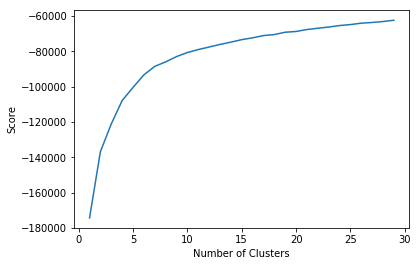
\includegraphics[scale=0.7]{2}
\end{center}

From the above graph, I took a safe value of 10 as the value of $\mathrm{M}$.

\begin{lstlisting}
k_cluster = 10

l2_lamda = 0.9

designMatrix = compute_design_matrix(X_train,k_cluster)
weights_train0 = closed_form_solution(l2_lamda, designMatrix, y_train)
train_error0 = rms_error(weights_train0,designMatrix,y_train,l2_lamda)
print("Training error:",train_error0)

designMatrix2 = compute_design_matrix(X_validate,k_cluster)
train_error2 = rms_error(weights_train0,designMatrix2,y_validate,l2_lamda)
print("Test error (Validation set):",train_error2)


#Test error
designMatrix3 = compute_design_matrix(X_test,k_cluster)
train_error3 = rms_error(weights_train0,designMatrix3,y_test,l2_lamda)
print("Test error (test set):",train_error3)
\end{lstlisting}


\section*{Code Output}

\begin{lstlisting}[label={list:fifth},caption=Code output.]
From closed form solution.
Training error: [[ 0.54948601]]
Test error (Validation set): [[ 0.64268395]]
Test error (test set): [[ 0.68269302]]
From SGD.
Training error: 0.560374755594
Test error (Validation set): 0.556667218125
Test error (test set): 0.639586215758
\end{lstlisting}

\vfill
\section*{Results 2}

The following plots are drawn to better understand and decide the variation between the 3 errors and hyper-parameters such as regularization $\lambda$ and learning rate $\eta$.

\begin{center}
	For Closed Form Solution
	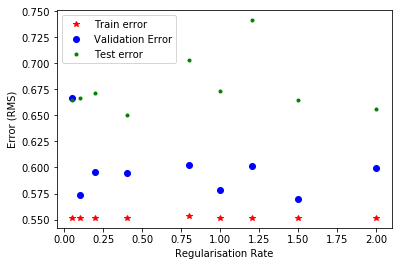
\includegraphics[scale=0.8]{3}
\end{center}
\begin{center}
	For Stochastic Gradient Descent
	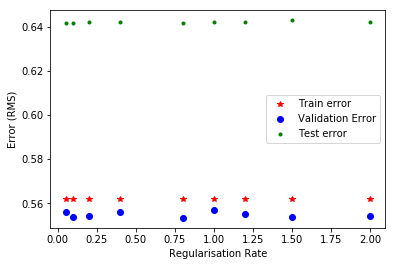
\includegraphics[scale=0.8]{4}
\end{center}\vfill
\begin{center}
	For Stochastic Gradient Descent
	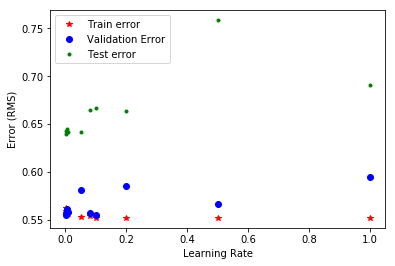
\includegraphics[scale=0.8]{5}
\end{center}

The below graphs are for the synthetic dataset.\\
\begin{center}
	For Closed Form Solution
	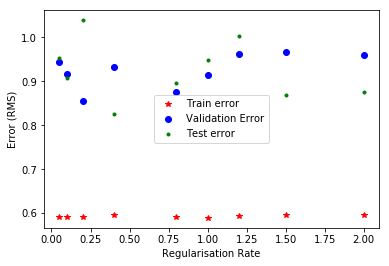
\includegraphics[scale=0.8]{B2}
\end{center}\vfill
\begin{center}
	For Stochastic Gradient Descent
	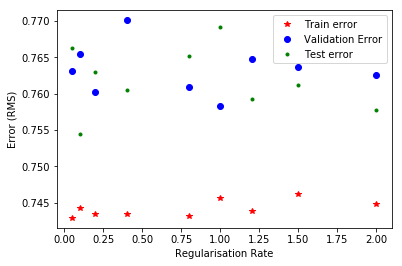
\includegraphics[scale=0.8]{B3}
\end{center}
\begin{center}
	For Stochastic Gradient Descent
	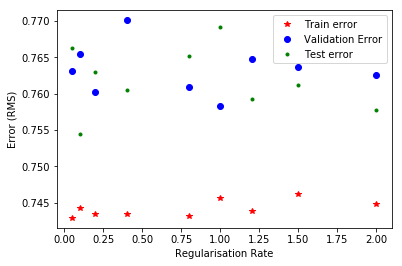
\includegraphics[scale=0.8]{B3}
\end{center}

\begin{itemize}
 \item The stochastic graient descent appears to have a better error rate than closed form solution even though test error is high when compared to train and validation set error but has a little consistency.
\item The learning time increases significantly with the increase in $\mathrm{M}$, the number of basis functions. 
\end{itemize}


\end{document}
